\documentclass[14pt, a4paper]{extarticle}

\usepackage{graphicx}
\usepackage{amsmath}
\usepackage{float}
\usepackage{wrapfig}

\usepackage{gvv-book}
\usepackage{gvv}



\graphicspath{{figs/}}
\renewcommand{\theequation}{1.9.13.\arabic{equation}}
\renewcommand{\thefigure}{1.9.13.\arabic{figure}}

\title{1.9.13}
\author{E Achyuta Siddartha - ee25btech11024}

\begin{document}
\maketitle

\section*{Problem Statement}
A man goes 5 meters due west and then 12 meters due north. How far is he from
the starting point?

\section*{Solution:}
Let's assume that the man starts from the origin. He moves 5 m west to point A.
\begin{align}
    \vec{A} = 5\myvec{-1 \\ 0}
\end{align}

He then moves 12m north from B.
\begin{align}
    \vec{B} = 5\myvec{-1 \\ 0} + 12\myvec{0 \\ 1} = \myvec{-5 \\ 12}
\end{align}

Therefore the corrdinates are

\begin{center}
    \begin{tabular}{|c|c|c|}
    \hline
    \textbf{Symbol} & \textbf{Value} & \textbf{Description}  \\
    \hline
    \textbf{\vec{0}}      & \myvec{0 \\ 0}         & Origin        \\
    \hline
    \textbf{\vec{A}}      & \myvec{-5 \\ 0}        & First Point   \\
    \hline
    \textbf{\vec{B}}      & \myvec{-5 \\ 12}      &Second Point    \\
    \hline
    \end{tabular}
\end{center}
\noindent
We need to find the distance between the starting point O and the final point B.

\begin{align}
    \vec{O} - \vec{B} = \myvec{0 \\ 0} - \myvec{-5 \\ 12} = \myvec{5 \\ -12}
\end{align}

\begin{align}
    (\vec{0} - \vec{B})^\top(\vec{0} - \vec{B}) = 169 = \|0 - B\|^2
\end{align}

Thus the desired distance is
\begin{align}
    d = \|\vec{O} - \vec{B}\| = \sqrt{169} = 13
\end{align}

The distance between the man and the starting point = 13 \\

See Figure~\ref{fig:pathofman}.

\begin{figure}[h!]
    \centering
    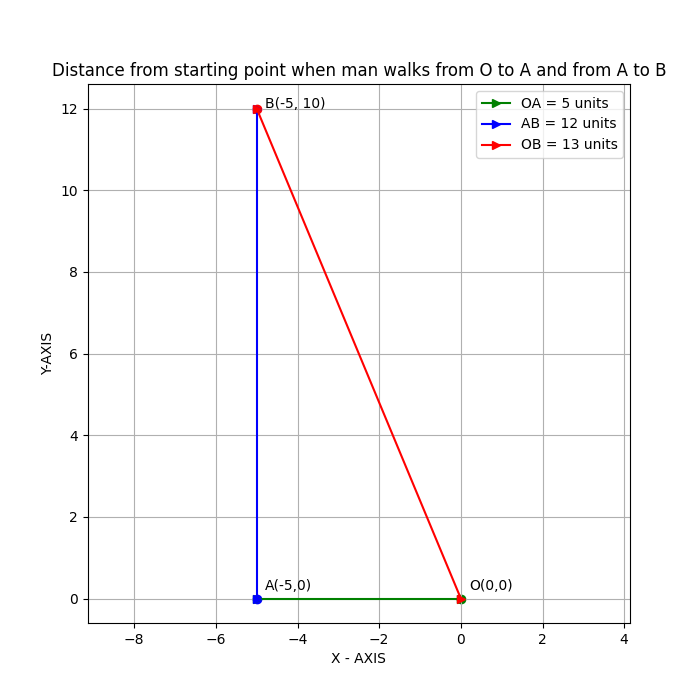
\includegraphics[width=0.8\linewidth]{figs/fig2.png}
    \caption{}
    \label{fig:pathofman}
\end{figure}

\end{document}